\section{Results}\label{sec:results}

\subsection{Compiled programs}\label{sec:res-programs}

Table~\ref{tab:programs} lists the compiled programs. The schedule of Section~\ref{sec:frame} adds no NOPs beyond
the padding for the distance 5 and 7 surface codes, whose layers hold many independent instructions; their slot
counts exceed the instruction counts by the second slots of the two qubit instructions. The distance 3
surface code needs a few NOPs and the repetition code, with five qubits, needs most of its slots as NOPs; both
programs are short, so a batch still takes only a few hundred cycles.

\begin{table}[t]
\caption{Compiled programs. Instructions excludes the NOPs inserted by the schedule. Slots, the cycles per batch of
the frame stage, counts one slot per single qubit instruction, two per two qubit instruction and one per NOP.
Columns: qubits after renumbering, instructions, two qubit (2q) instructions, NOPs, slots, measurements,
outputs (detectors plus observables) and fold entries.}\label{tab:programs}
% generated by scripts/make_numbers.py
\begin{tabular}{@{}lrrrrrrrr@{}}
\toprule
Circuit & Qubits & Instr. & 2q & NOPs & Slots & Meas. & Out. & Fold \\
\midrule
Repetition code, $d=3$ & 5 & 44 & 12 & 74 & 130 & 9 & 9 & 17 \\
Surface code, $d=3$ & 17 & 343 & 144 & 28 & 515 & 33 & 25 & 55 \\
Surface code, $d=5$ & 49 & 1{,}673 & 800 & 16 & 2{,}489 & 145 & 121 & 261 \\
Surface code, $d=7$ & 97 & 4{,}667 & 2{,}352 & 16 & 7{,}035 & 385 & 337 & 715 \\
\botrule
\end{tabular}

\end{table}

\subsection{Synthesis and implementation}\label{sec:res-impl}

All loops of the kernel were scheduled by Vitis HLS with an initiation interval of one cycle, and HLS estimated a
maximum clock of \NumHlsFmax{}~MHz for a target of 300~MHz. Placing and routing the kernel on the card was the
difficult step. Table~\ref{tab:builds} lists every implementation run, each with two instances at 300~MHz. The
\NumFailedBuilds{} runs with the Philox noise stage all failed Vivado's verification of the routed design with
conflicting nets, after about five hours each: first with the frame in registers, then with the frame in LUT RAM, and
then also with a placement directive that spreads logic to relieve congestion. The congestion analysis of the first
run (Section~\ref{sec:frame}) explains the pattern: removing the register crossbar removed the short range hot spots,
but the noise stage with \NumPhiloxDsp{} DSP blocks per instance still filled the DSP columns of its region, and in
all three runs every one of the ten conflicting nets that Vivado lists lay in the instance placed in SLR0, which it
shares with the platform's HBM and DMA logic. Replacing Philox by Threefry removed the DSP demand (\NumHlsDsp{} DSP blocks per instance), and the
instances were moved to SLR1 and SLR2. With both changes the design routed: the placer no longer reported the
design as congested, and the run with the standard placement directive met timing at 300~MHz with a worst negative
slack of \NumWns{}~ns after \NumTfImplTime{} of implementation, less than half the time of each failed run. The
parallel run with the spreading directive was stopped once this result was available.

\begin{table}[t]
\caption{Implementation runs of the kernel on the Alveo U55C, two instances at a 300~MHz target. Frame: frame stage
storage. Generator: Philox4x32-10 or Threefry4x32-20. SLRs: the regions of the two instances. Placement: Vivado
directive ExtraTimingOpt (timing) or AltSpreadLogic\_high (spread). DSP: DSP blocks per instance (HLS). Time: Vivado
placement and routing. All runs used the
same post route optimisation settings.}\label{tab:builds}
% generated by scripts/make_numbers.py
\begin{tabular}{@{}llllrrl@{}}
\toprule
Frame & Generator & SLRs & Placement & DSP & Time & Outcome \\
\midrule
registers & Philox & 0, 1 & timing & 2{,}076 & 5~h 18~min & routing failed \\
LUT RAM & Philox & 0, 1 & timing & 2{,}076 & 4~h 55~min & routing failed \\
LUT RAM & Philox & 0, 1 & spread & 2{,}076 & 5~h 23~min & routing failed \\
LUT RAM & Threefry & 1, 2 & timing & 12 & 2~h 04~min & bitstream \\
LUT RAM & Threefry & 1, 2 & spread & 12 & stopped & stopped \\
\botrule
\end{tabular}

\end{table}

Table~\ref{tab:resources} compares the HLS estimate of one instance with the routed design. The HLS estimate of logic is
conservative: a routed instance uses \NumRoutedLutOne{} LUTs
against \NumHlsLut{} estimated. The routed design runs at \NumKernelMhz{}~MHz with a worst negative slack of
\NumWns{}~ns.

\begin{table}[t]
\caption{Resources of the kernel. HLS: estimate for one instance, in percent of one SLR. Routed: one instance, and
all \NumInstancesPerCard{} instances of a card in percent of the resources available to user logic, from the post
route utilisation report.}\label{tab:resources}
% generated by scripts/make_numbers.py
\begin{tabular}{@{}lrrrr@{}}
\toprule
Resource & HLS, one instance & \% SLR & Routed, one instance & Routed, card (\% budget) \\
\midrule
LUT & 145{,}414 & 33 & 80{,}941 & 161{,}975 (13.76) \\
FF & 82{,}131 & 9 & 61{,}272 & 122{,}546 (5.06) \\
DSP & 12 & 0 & 12 & 24 (0.27) \\
\botrule
\end{tabular}

\end{table}

RTL cosimulation of the distance 3 surface code took \NumCosimCyclesA{} cycles for \NumCosimBatchesA{} batches and
\NumCosimCyclesB{} cycles for \NumCosimBatchesB{}, that is \NumCosimPerBatch{} cycles per additional batch for a
program of \NumSlotsSurfThree{} slots. The four stages keep pace with each other: the frame stage completes one slot
per cycle, and a batch costs \NumCosimOverhead{} cycles more than its slots.

\subsection{Correctness on hardware}\label{sec:res-correct}

Every kernel instance of every card produced output bit identical to the software model for the three benchmark
circuits (\NumBenchCheckPassed{} of \NumBenchCheckTotal{} card and circuit checks). Table~\ref{tab:tier4} gives the
Tier 4 comparison with Stim and Table~\ref{tab:ler} the Tier 5 logical error rates. All outputs of all circuits agree
with Stim within the $5\sigma$ bound (largest $|z|$ \NumTierFourMaxZ{}), and the decoded logical error rates of
hardware and Stim samples agree at every distance and error rate (largest $|z|$ \NumTierFiveMaxZ{}). The rates show
the expected behaviour of the surface code: below threshold the logical error rate falls with distance, at
$p=0.01$ it rises.

\begin{table}[t]
\caption{Tier 4: detector and observable firing rates of hardware samples against Stim. The largest two proportion
$|z|$ over all outputs of a circuit is reported.}\label{tab:tier4}
% generated by scripts/make_numbers.py
\begin{tabular}{@{}lrrr@{}}
\toprule
Circuit & FPGA shots & Stim shots & max $|z|$ \\
\midrule
Repetition code, $d=3$ & 10{,}223{,}616 & 10{,}000{,}000 & 1.43 \\
Surface code, $d=3$ & 10{,}223{,}616 & 10{,}000{,}000 & 3.12 \\
Surface code, $d=5$ & 10{,}223{,}616 & 10{,}000{,}000 & 2.74 \\
\botrule
\end{tabular}

\end{table}

\begin{table}[t]
\caption{Tier 5: logical error rates (LER) of rotated surface code memory experiments, hardware samples against Stim
samples, both decoded by the same PyMatching matcher.}\label{tab:ler}
% generated by scripts/make_numbers.py
\begin{tabular}{@{}rrrrrr@{}}
\toprule
$d$ & $p$ & Shots & FPGA LER & CPU Stim LER & $z$ \\
\midrule
3 & 0.001 & 1{,}048{,}576 & 7.753e-04 & 7.734e-04 & $+0.05$ \\
3 & 0.003 & 1{,}048{,}576 & 6.518e-03 & 6.616e-03 & $-0.87$ \\
3 & 0.010 & 1{,}048{,}576 & 5.939e-02 & 5.908e-02 & $+0.97$ \\
5 & 0.001 & 1{,}048{,}576 & 1.402e-04 & 1.373e-04 & $+0.18$ \\
5 & 0.003 & 1{,}048{,}576 & 3.340e-03 & 3.286e-03 & $+0.67$ \\
5 & 0.010 & 1{,}048{,}576 & 8.339e-02 & 8.377e-02 & $-0.99$ \\
7 & 0.001 & 1{,}048{,}576 & 1.621e-05 & 2.289e-05 & $-1.09$ \\
7 & 0.003 & 1{,}048{,}576 & 1.466e-03 & 1.533e-03 & $-1.25$ \\
7 & 0.010 & 1{,}048{,}576 & 1.034e-01 & 1.032e-01 & $+0.39$ \\
\botrule
\end{tabular}

\end{table}

\subsection{Throughput on one, two and four nodes}\label{sec:res-throughput}

Table~\ref{tab:throughput} and Figure~\ref{fig:throughput} give the measured sampling rates. One card with
\NumInstancesPerCard{} instances samples the distance 5 surface code at \NumFpgaOneSurfFive{} shots per second, and four
cards at \NumFpgaFourSurfFive{}. Going from one to four nodes multiplies the rate by \NumScaleFactorMin{} to
\NumScaleFactorMax{} over the three circuits, that is, the nodes scale linearly: they share nothing but the host,
and at these output volumes the host side (launching, copying results to host memory, synchronising the processes)
does not limit the rate. The per card rates within a run differ by less than one percent. The FPGA temperatures read before and after
every configuration were at most \NumMaxFpgaTemp{}~\textdegree C.

\begin{table}[t]
\caption{Sampling rates in shots per second (median of \NumBenchReps{} runs) on one, two and four cards. $S_4$: four
card rate over one card rate. $R_1$, $R_{\mathrm{all}}$: four card rate over Stim on the same host with one process
and with \NumCpuMaxProcs{} processes (Table~\ref{tab:cpu}). All rates count only shots whose outputs have reached host
memory.}\label{tab:throughput}
% generated by scripts/make_numbers.py
\begin{tabular}{@{}lrrrrrr@{}}
\toprule
Circuit & 1 card & 2 cards & 4 cards & $S_4$ & $R_1$ & $R_{\mathrm{all}}$ \\
\midrule
Repetition code, $d=3$ & 289{,}230{,}495 & 577{,}517{,}899 & 1{,}155{,}366{,}309 & 3.99$\times$ & 193$\times$ & 8.24$\times$ \\
Surface code, $d=3$ & 73{,}912{,}169 & 147{,}798{,}429 & 295{,}658{,}952 & 4.00$\times$ & 104$\times$ & 2.39$\times$ \\
Surface code, $d=5$ & 15{,}338{,}202 & 30{,}687{,}981 & 61{,}359{,}029 & 4.00$\times$ & 84.8$\times$ & 1.07$\times$ \\
\botrule
\end{tabular}

\end{table}

\begin{figure}[t]
\centering
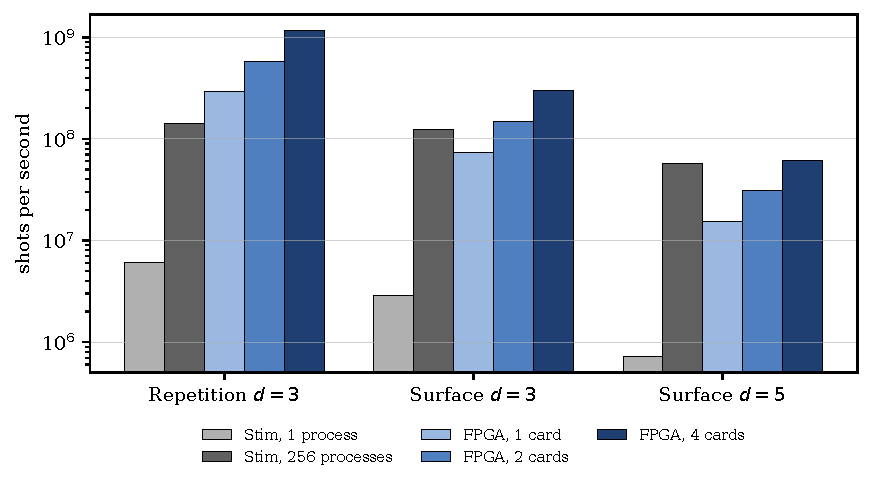
\includegraphics[width=0.85\textwidth]{figures/fig_throughput.pdf}
\caption{Sampling rate of the three benchmark circuits on one, two and four cards, and of Stim with one process and
with all hardware threads of the host. Logarithmic scale.}\label{fig:throughput}
\end{figure}

\begin{table}[t]
\caption{Stim~\NumStimVersion{} on the host: shots per second with $P$ concurrent processes.}\label{tab:cpu}
% generated by scripts/make_numbers.py
\begin{tabular}{@{}lrrrrr@{}}
\toprule
Circuit & 1 proc. & 16 proc. & 64 proc. & 128 proc. & 256 proc. \\
\midrule
Repetition code, $d=3$ & 5{,}999{,}732 & 60{,}814{,}996 & 84{,}704{,}275 & 100{,}987{,}950 & 140{,}258{,}256 \\
Surface code, $d=3$ & 2{,}841{,}093 & 35{,}270{,}693 & 65{,}480{,}163 & 78{,}332{,}218 & 123{,}750{,}688 \\
Surface code, $d=5$ & 723{,}625 & 10{,}181{,}623 & 26{,}614{,}558 & 35{,}169{,}041 & 57{,}200{,}963 \\
\botrule
\end{tabular}

\end{table}

Against one Stim process, the four node system is faster by the factors in Table~\ref{tab:throughput}
(\NumRatioOneSurfFive{} times for the distance 5 surface code). The more demanding comparison is with Stim on all
\NumHostThreads{} hardware threads of the same host: there the four node system reaches \NumRatioAllSurfFive{} times
the CPU rate for the distance 5 surface code, \NumRatioAllSurfThree{} times for the distance 3 surface code and
\NumRatioAllRep{} times for the repetition code. Stim's rate grows less than linearly with the number of processes
(Table~\ref{tab:cpu}); we did not investigate the cause on this host.

\subsection{Comparison with the first kernel and with the cycle model}\label{sec:res-first}

On one card the first kernel sampled the three circuits at \NumFirstKernelRep{}, \NumFirstKernelSurfThree{} and
\NumFirstKernelSurfFive{} shots per second (Section~\ref{sec:first}), measured at a 250~MHz kernel clock on the
project's build host, whose CPU is the same model. The new kernel on one card is faster by factors of
\NumOverFirstRep{}, \NumOverFirstSurfThree{} and \NumOverFirstSurfFive{}. The cycle count of the kernel predicts the
rate of a card from the program alone: an instance delivers \NumLanes{} shots per batch, and a batch takes as many
cycles as the largest of its slot count, its measurement and fold work, and its output count, so a card should
sample at \NumModelCardRep{}, \NumModelCardSurfThree{} and \NumModelCardSurfFive{} shots per second. The measured one
card rates are \NumModelFracRep\,\%, \NumModelFracSurfThree\,\% and \NumModelFracSurfFive\,\% of these predictions; the
remainder is launch overhead and the copy of results to host memory, which weigh most for the short repetition code
program.
